\subsubsection{Bucket}

  \begin{enumerate}
    \item The main requirements for the module were:
  	  \begin{itemize}
        \item Maximum capacity: five cubes and three spheres
        \item A mechanical limiter on the amount of debris in the bucket 
        \item A closing mechanism for the bucket
        \item Delivery mechanism for putting the debris into the goals.  содержимое...
  	  \end{itemize}  
    \item The first stage of development was creating the general concept of the module, its structure and method of operation. In result, was decided on the following mechanism: 
    The bucket is shifted outside of the robot and turned 90 degrees around an axis parallel to the axis of shift;
    both movements are done by one servo.
    This allows to place the bucket opening to be parallel to the ground and increase the accuracy of debris delivery. Movement in two planes at once is accomplished through sloped guide rails, which turn the beams with the bucket during their sideways movement. To prevent premature release of debris from the bucket, the bucket opening will be closed. 
    
  \item The next step was developing the closing mechanism. To minimize the load on the servo completing the turning movement, the center of mass of the module has to be situated as close as possible to the mounting point on the lifting mechanism. Thus, the following system was developed:
    \begin{itemize}
      \item On the beam which is mounted to the lifting mechanism, is installed a reel with twine.
      \item The twine is fixed in such a way that when the reel turns in one direction, one of the ends is pulled taut while the other  slacks, and vice versa.
      \item The twine wraps around several fixed blocks along all the beams which support the bucket.
      \item Above the bucket opening there is another axis with another reel identical to the first, and the surface which blocks the opening.
   \end{itemize} 
  This allows to open and close the bucket without adding any additional significant load on the servo which turns it. To make sure that such a mechanism for transmitting rotational movement indeed works, a simplified model was assembled. The results of our tests showed that this transmission is operable, but the angle between the extreme positions is slightly more than 135 degrees, rather than 180 degrees, but this is still enough to complete the task. 
  \item After that the parameters of the guiding rails (slope relative to the vertical direction, maximum height) were calculated depending on where they are mounted: 
  \begin{figure}[h]
  	\begin{minipage}[h]{1\linewidth}
  	    \center{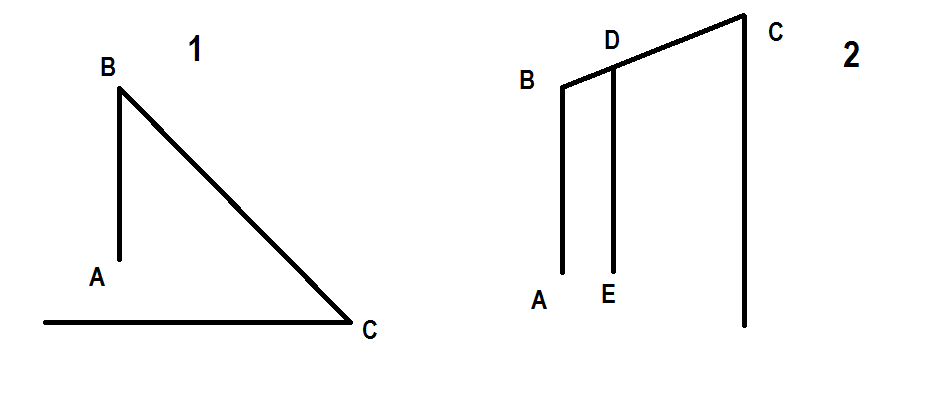
\includegraphics[scale = 0.4]{3Engineering/6Specifications_for_modules/bucket/images/01}}
   	    \caption{Side view of beams onto which the bucket is mounted}
   	\end{minipage}
  \end{figure}	
  The bucket, mounted on the beams, which in turn are mounted on the slats are in point A and move together. CB can rotate around point B. DE is the maximum height of the guiding rails. 
  Position 1: the bucket is lying on the ground and collecting debris. Position 2: the bucket is perpendicular to the ground and can deliver the debris to the goals. The needed ratios can be found from the easily derived formula: $<C = АЕ/(DE - BA)$.
  \item At the time the above process was completed, the qualification rounds were not far away, and so was decided to temporarily use two servos for shifting and turning the bucket, since the structure of the module would become significantly simpler and would require less time to complete. Were connected two slats in such a way that their uppermost part could move in both directions. After that on one of the ends of the slats were added limiters that depending on their position do not let one of the slats move. This does not prevent the robot from working properly, as we know our alliance before the match and thus in which direction we need to extend the bucket. This means we can adjust the limiters before the match.
  \begin{figure}[h]
  	\begin{minipage}[h]{1\linewidth}
  		\center{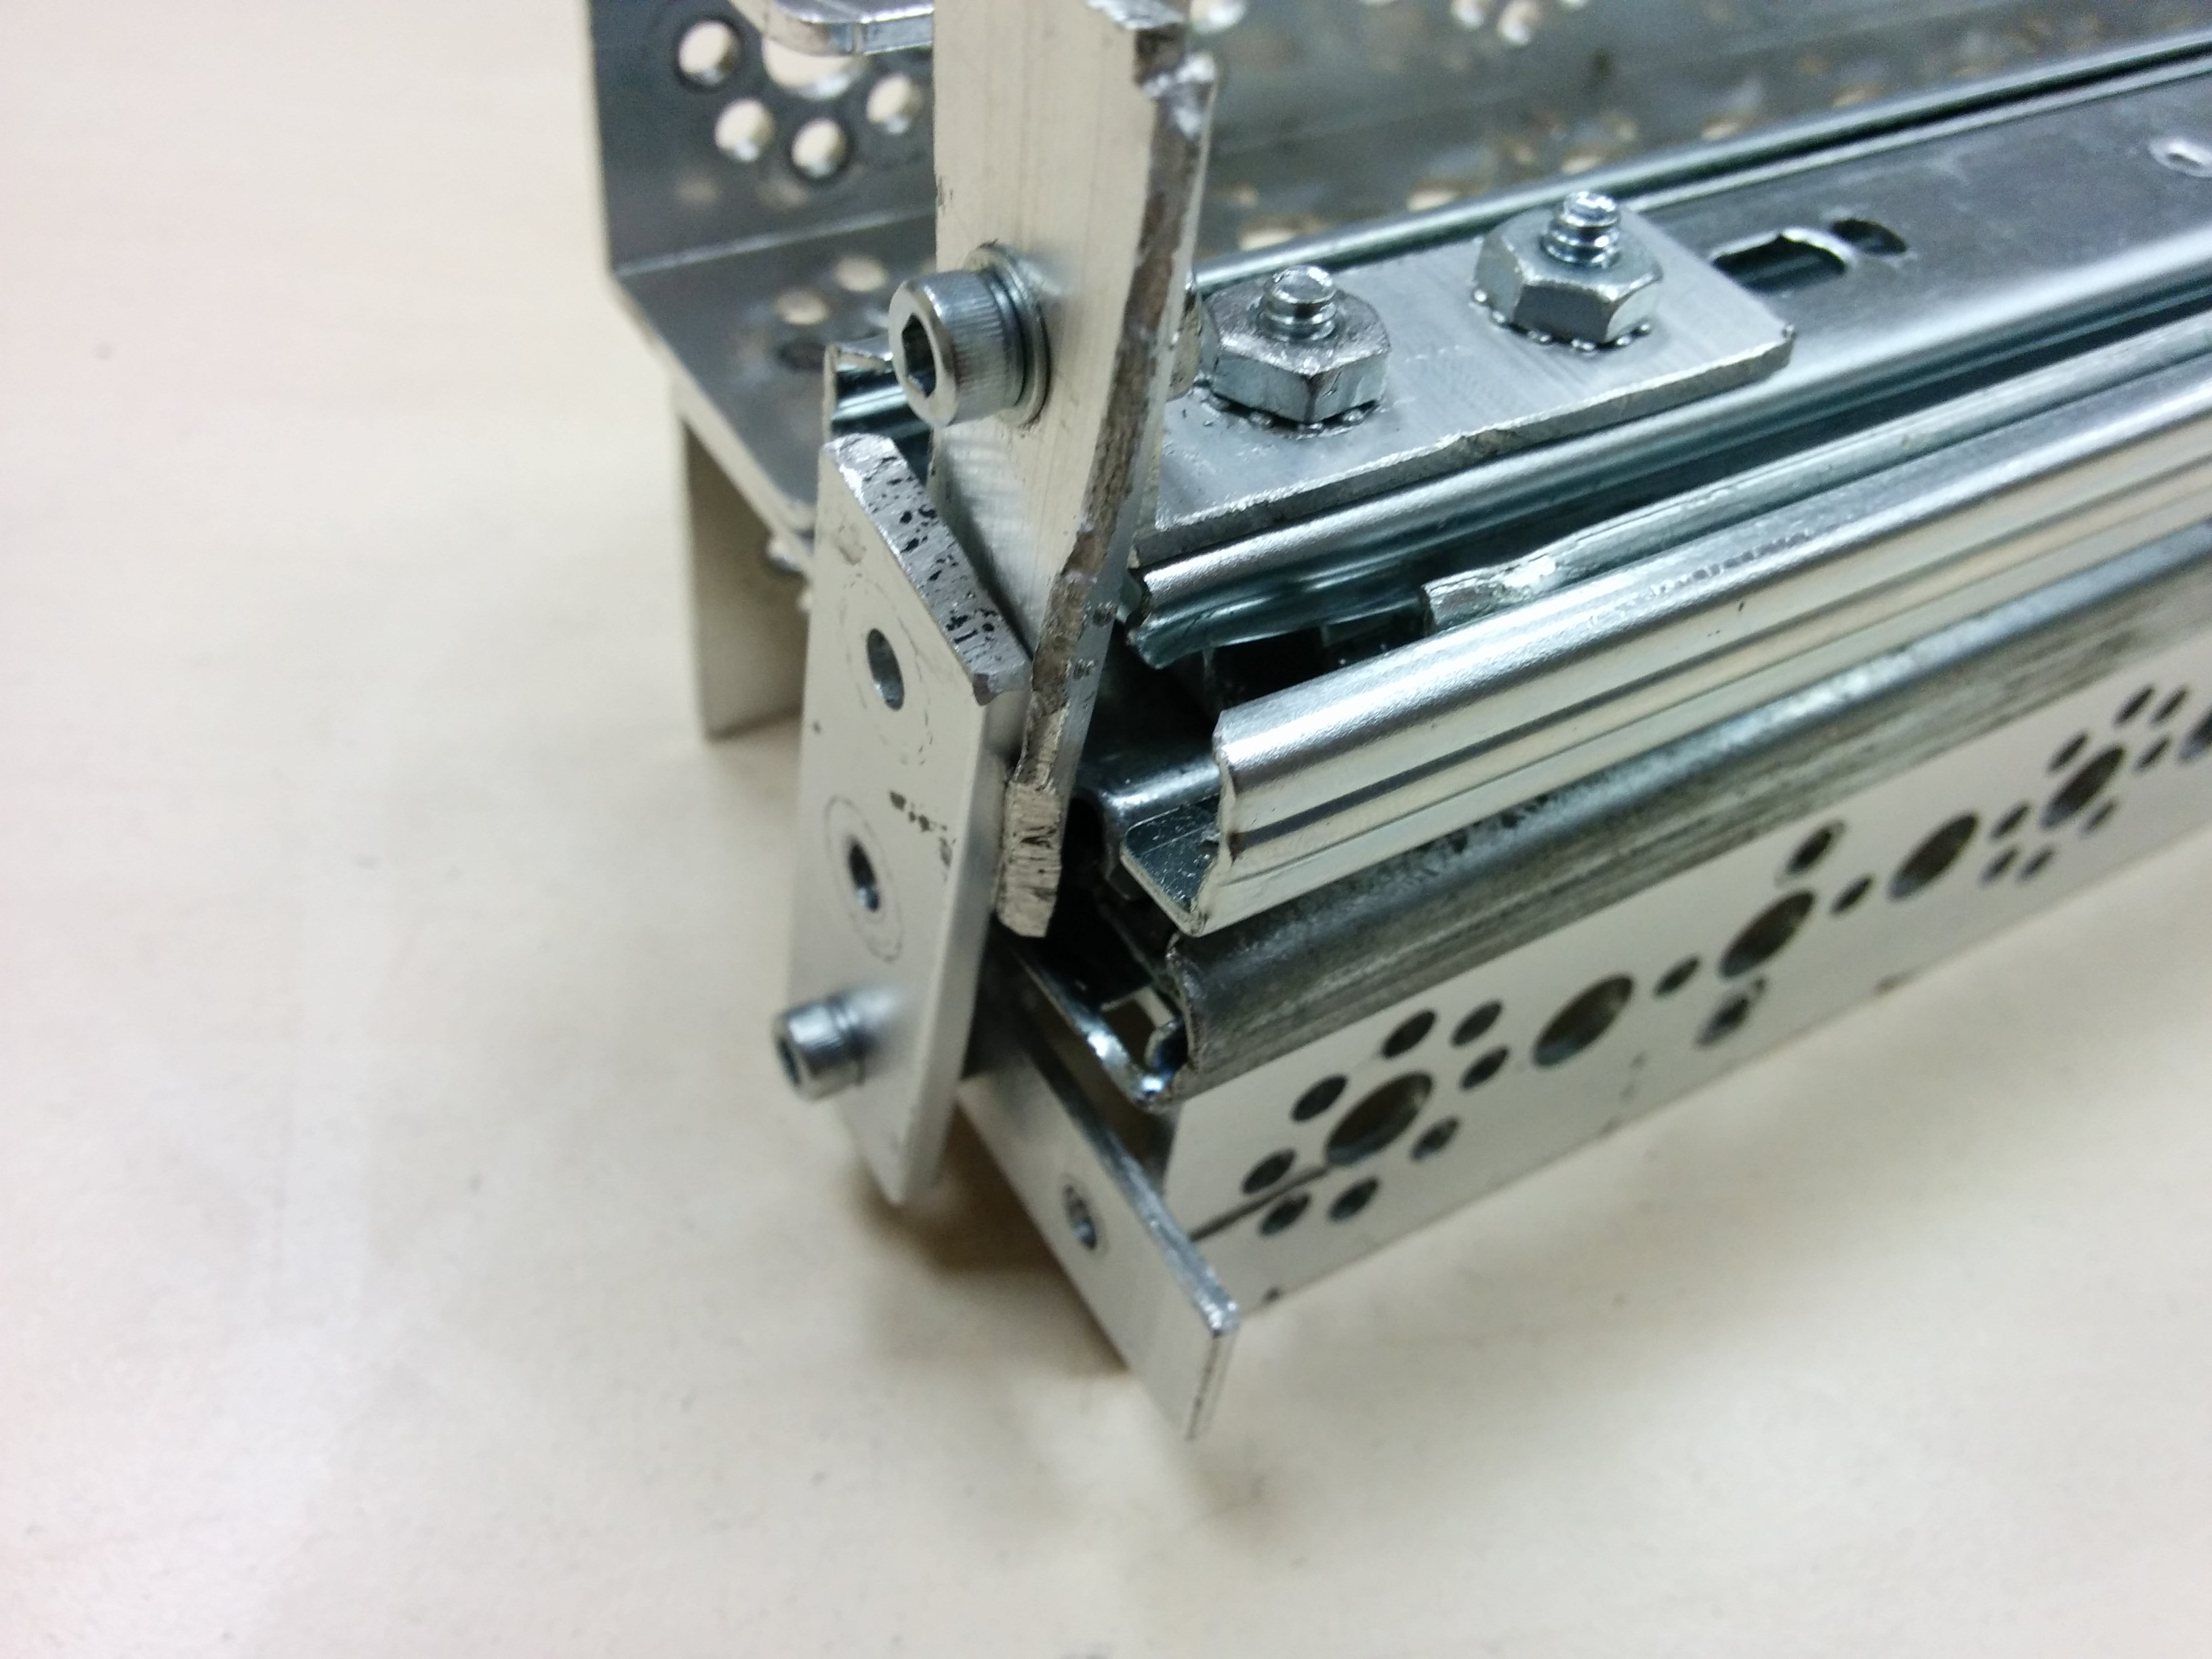
\includegraphics[scale = 0.05]{3Engineering/6Specifications_for_modules/bucket/images/02}}
  		\caption{Structure of limiters}
  	\end{minipage}
  \end{figure}
  (Note: in the figure both limiters are set to the closed position, in which neither slat can move; during the game itself one of the limiters will be set in the open position). 
  
  \item Then the servo with а reel for the twine moving the slats was fixed on. Blocks were attached to the ends of the fixed beams and wound the twine around them; the ends of the twine are tied to the ends of the slats, which allows them to move as needed. The servo direction of rotation defines the direction of movement of the slats and the bucket. 	
  
  \item After that was come up, tested and made another, less complicated, trapezoidal bucket with the opened part smaller than closed. The construction of the guides on the top of bucket would make debris fall in sequence 2-2-1 from the bottom, that way the scoring goals will hold maximum number of debris.
  \begin{figure}[h]
  	\begin{minipage}[h]{0.31\linewidth}
  		\center{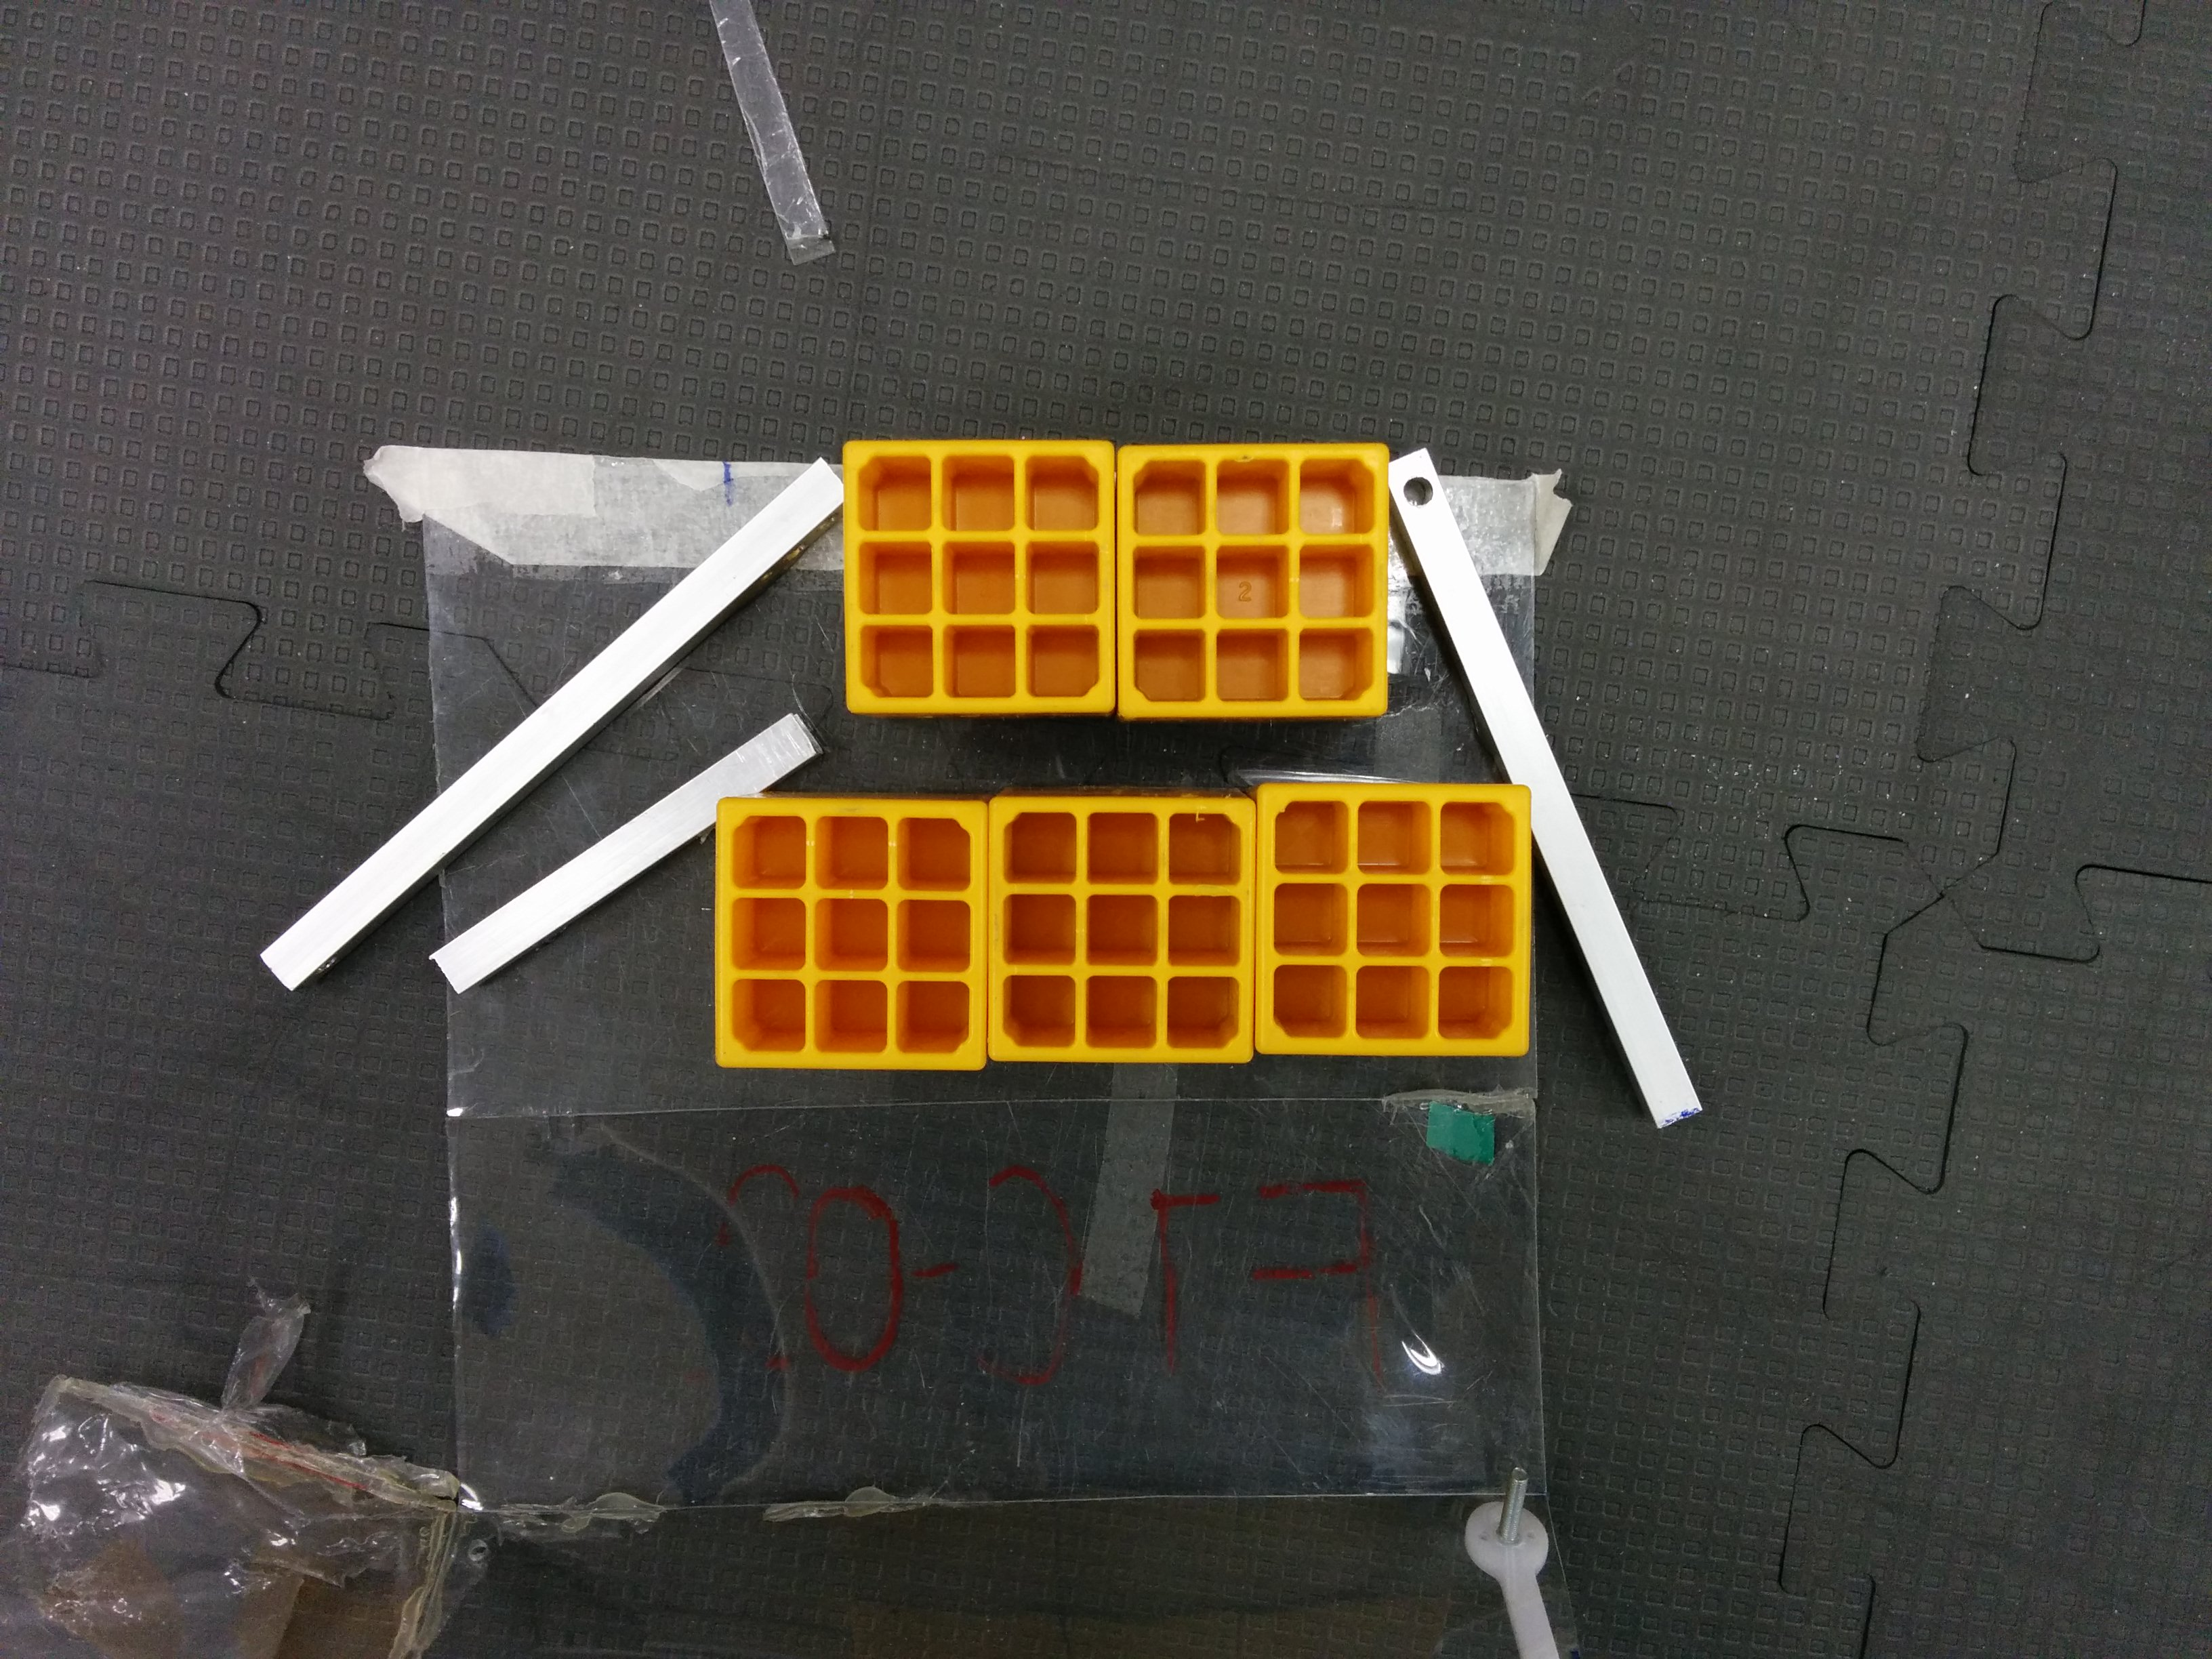
\includegraphics[scale = 0.04]{3Engineering/6Specifications_for_modules/bucket/images/03}}
  		\caption{Structure of guides}
  	\end{minipage}
  	\hfill
  	\begin{minipage}[h]{0.31\linewidth}
  		\center{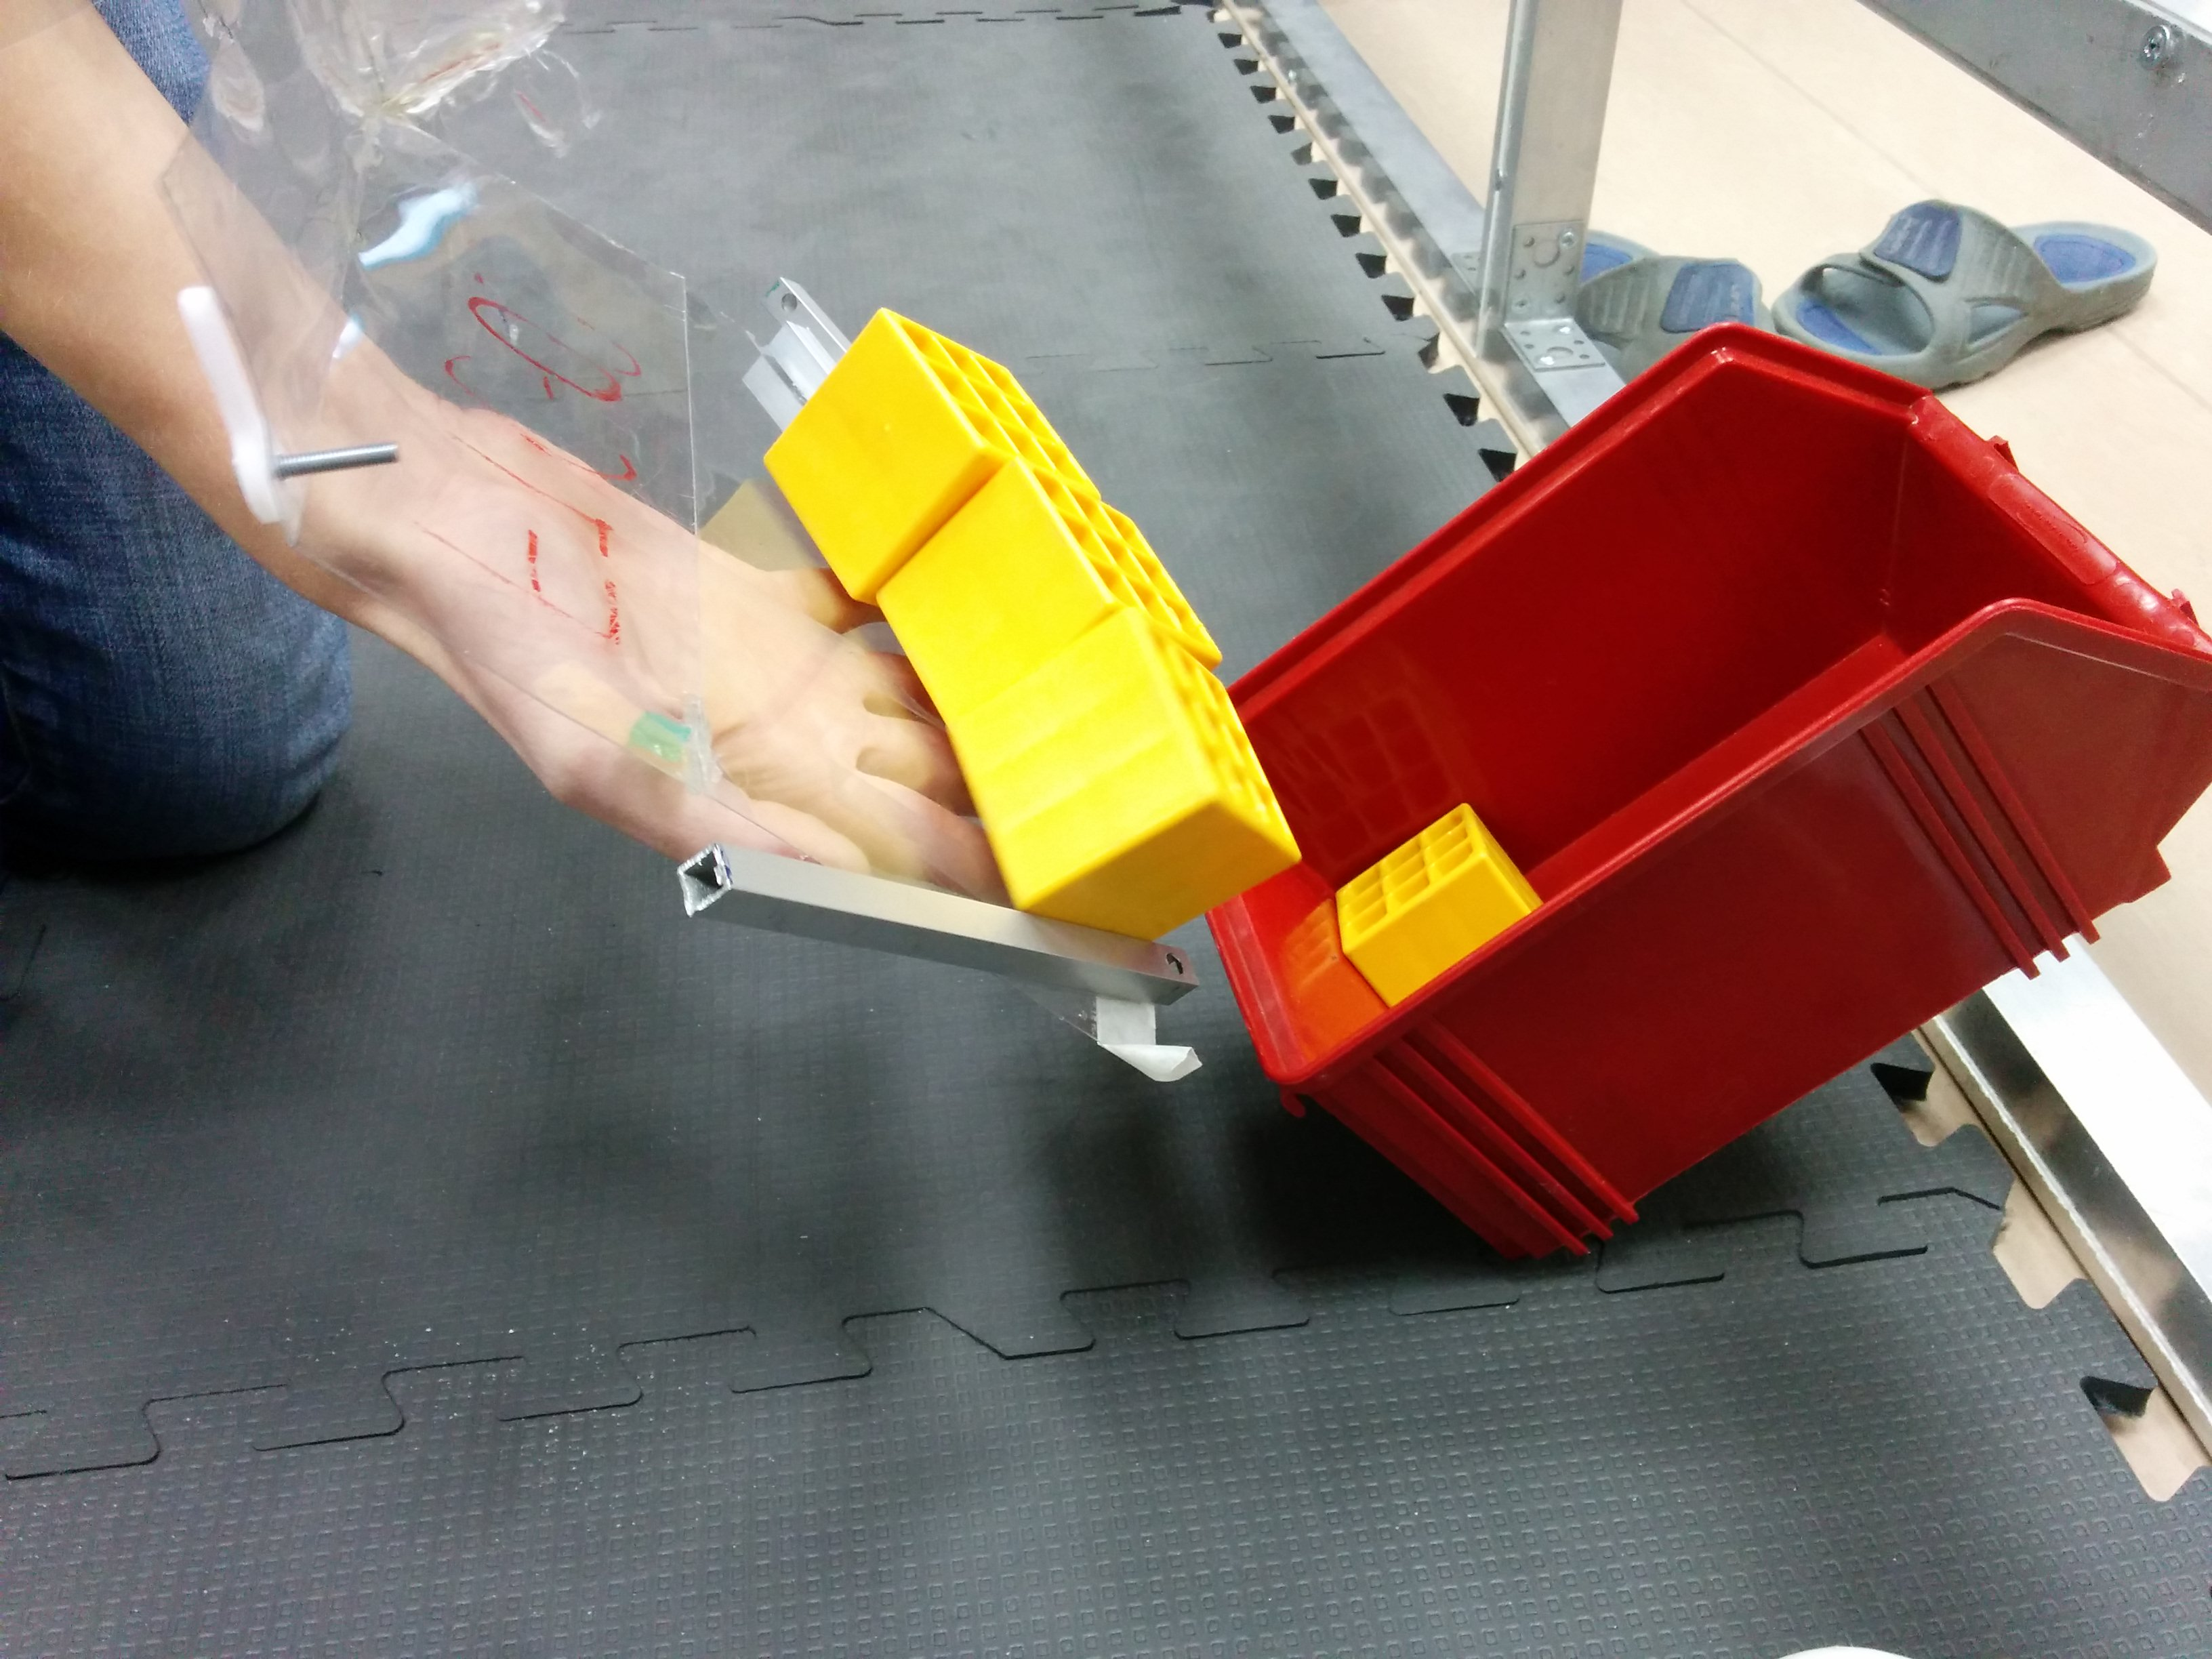
\includegraphics[scale = 0.04]{3Engineering/6Specifications_for_modules/bucket/images/04}}
  		\caption{Process of guides testing}
  	\end{minipage}
  	\hfill
  	\begin{minipage}[h]{0.31\linewidth}
  		\center{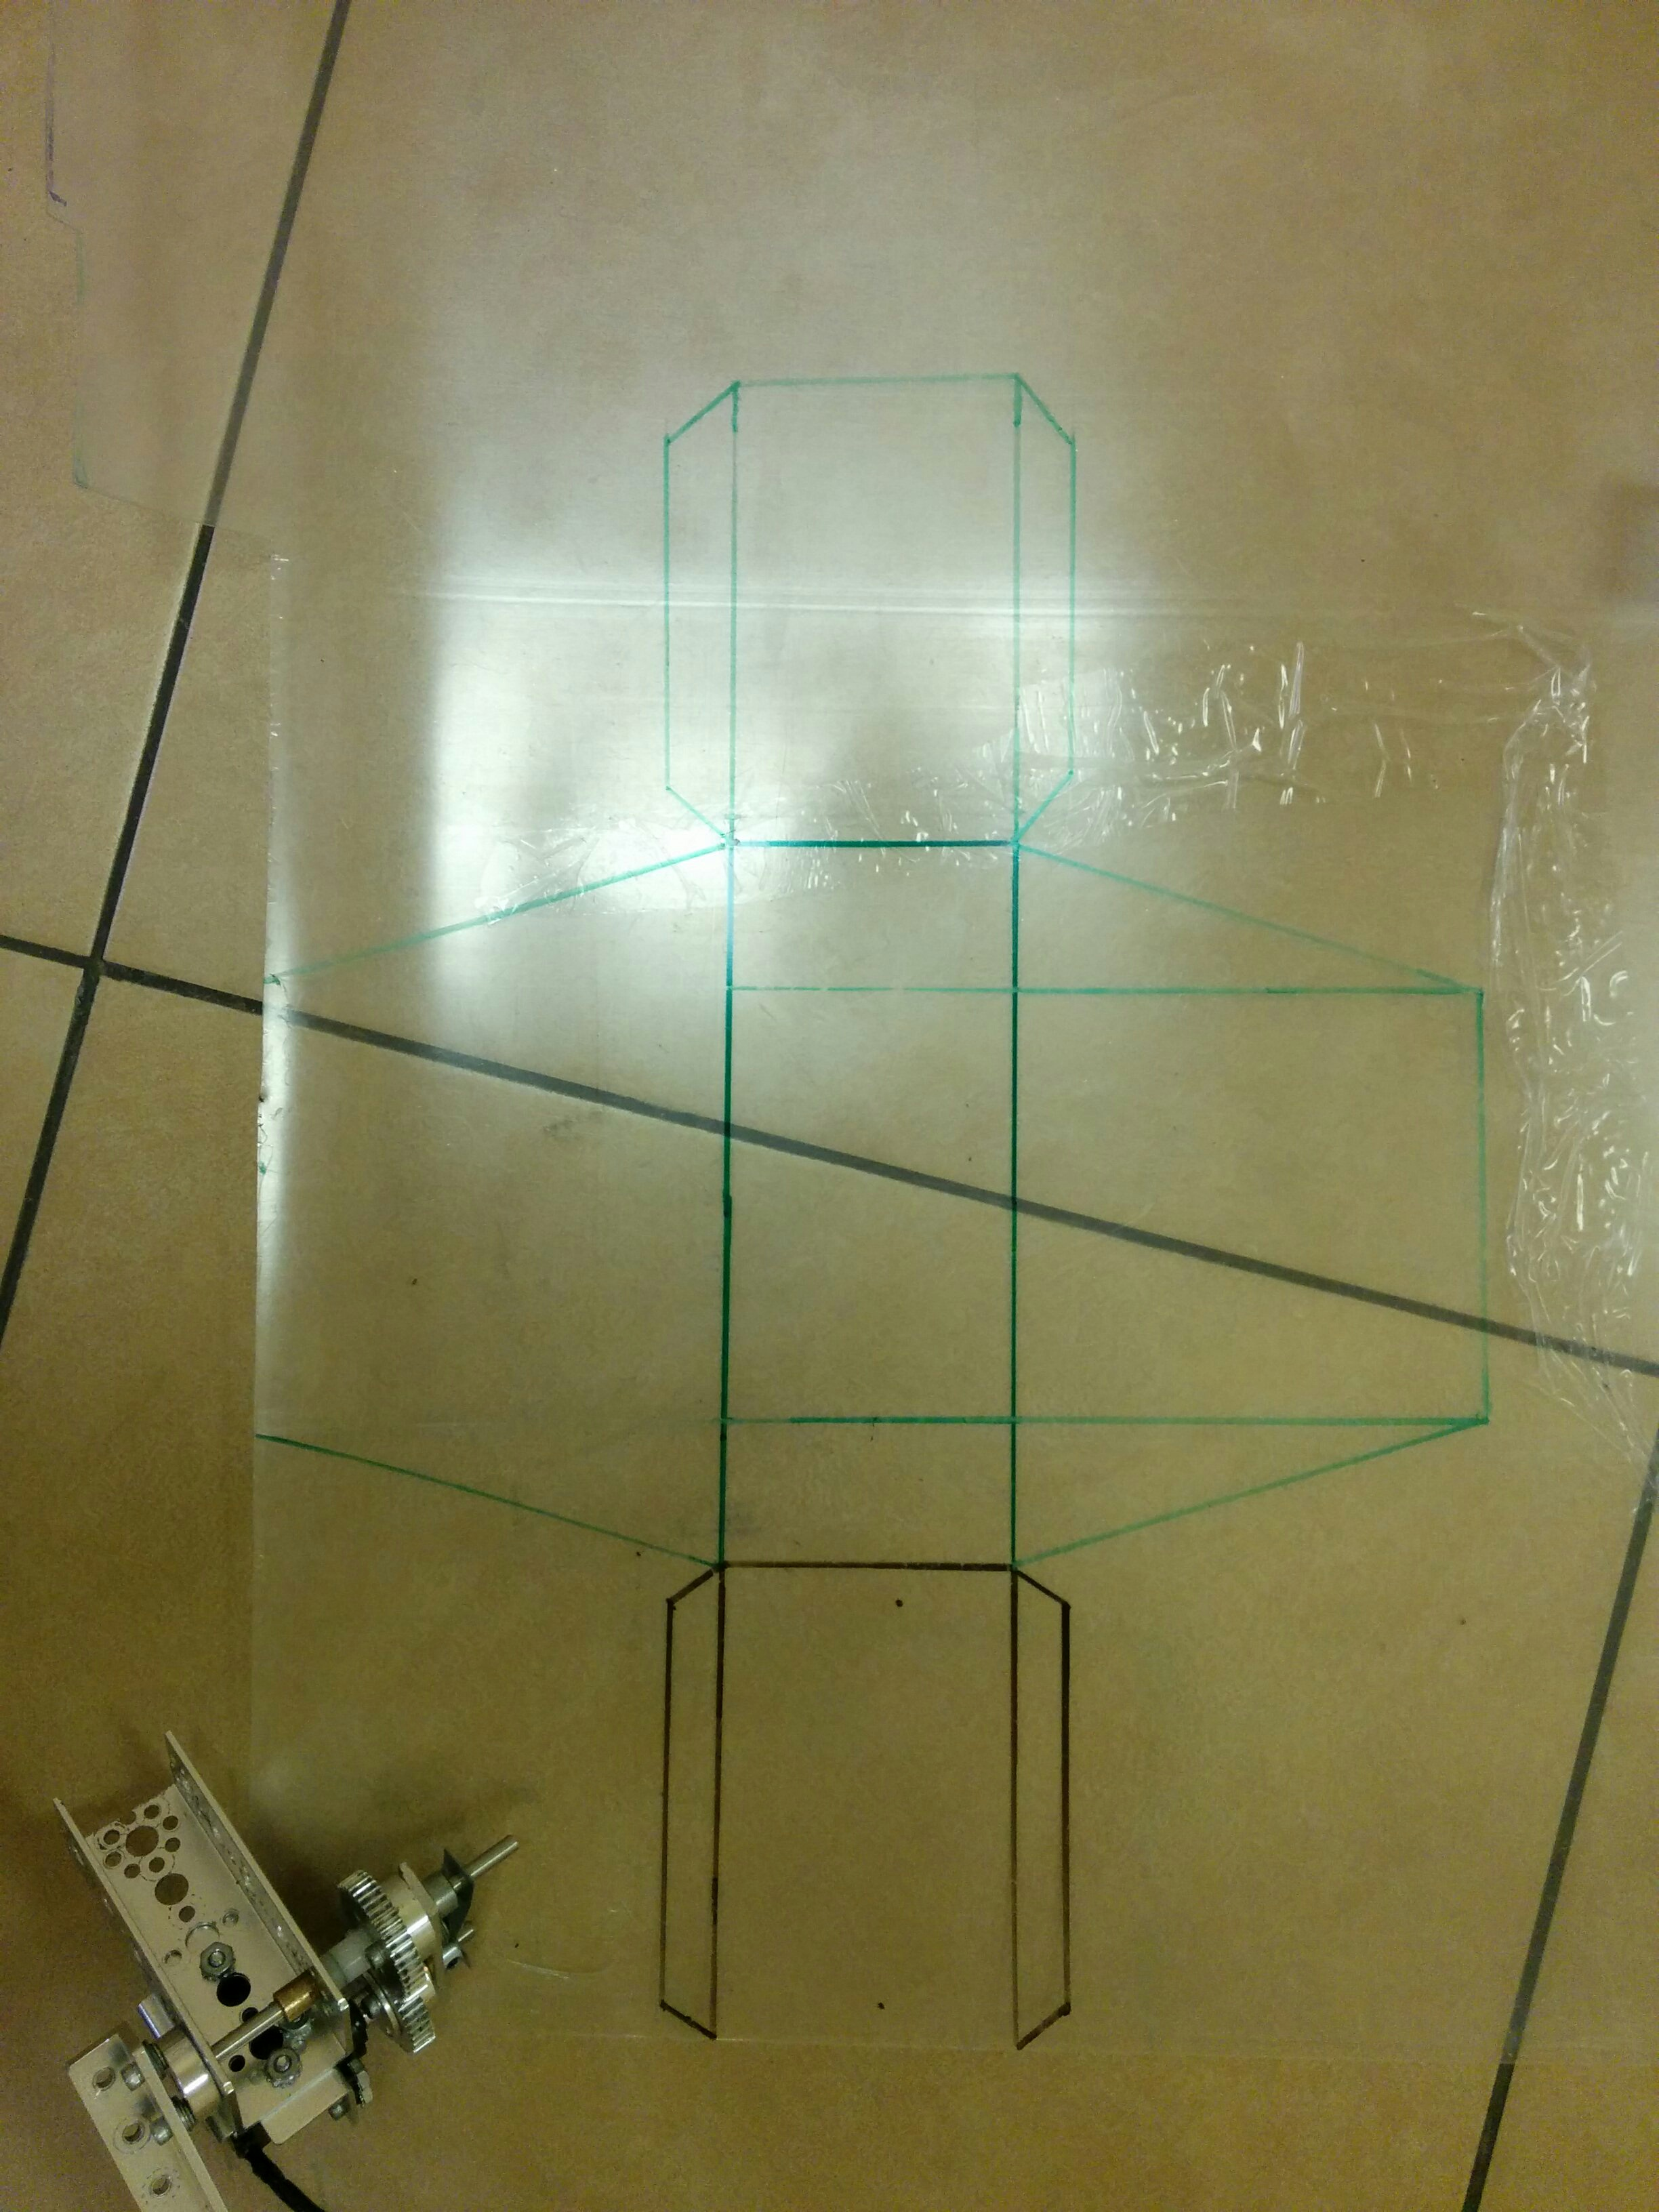
\includegraphics[scale = 0.04]{3Engineering/6Specifications_for_modules/bucket/images/05}}
  		\caption{Marking of bucket}
  	\end{minipage}
  \end{figure}
  Tests showed that guides work well, so was decided to use them in construction of bucket. The pair of front makes debris fall to the scoring goals more accurately, the assymetric guide slows one debri to make all the debris fall as 2-2-1, not 2-3.
 
  \item After that was streched the line to move the slats. Servos for moving the slats and turning the bucket were placed on the slats.
  \begin{figure}[h]
  	\begin{minipage}[h]{0.47\linewidth}
  		\center{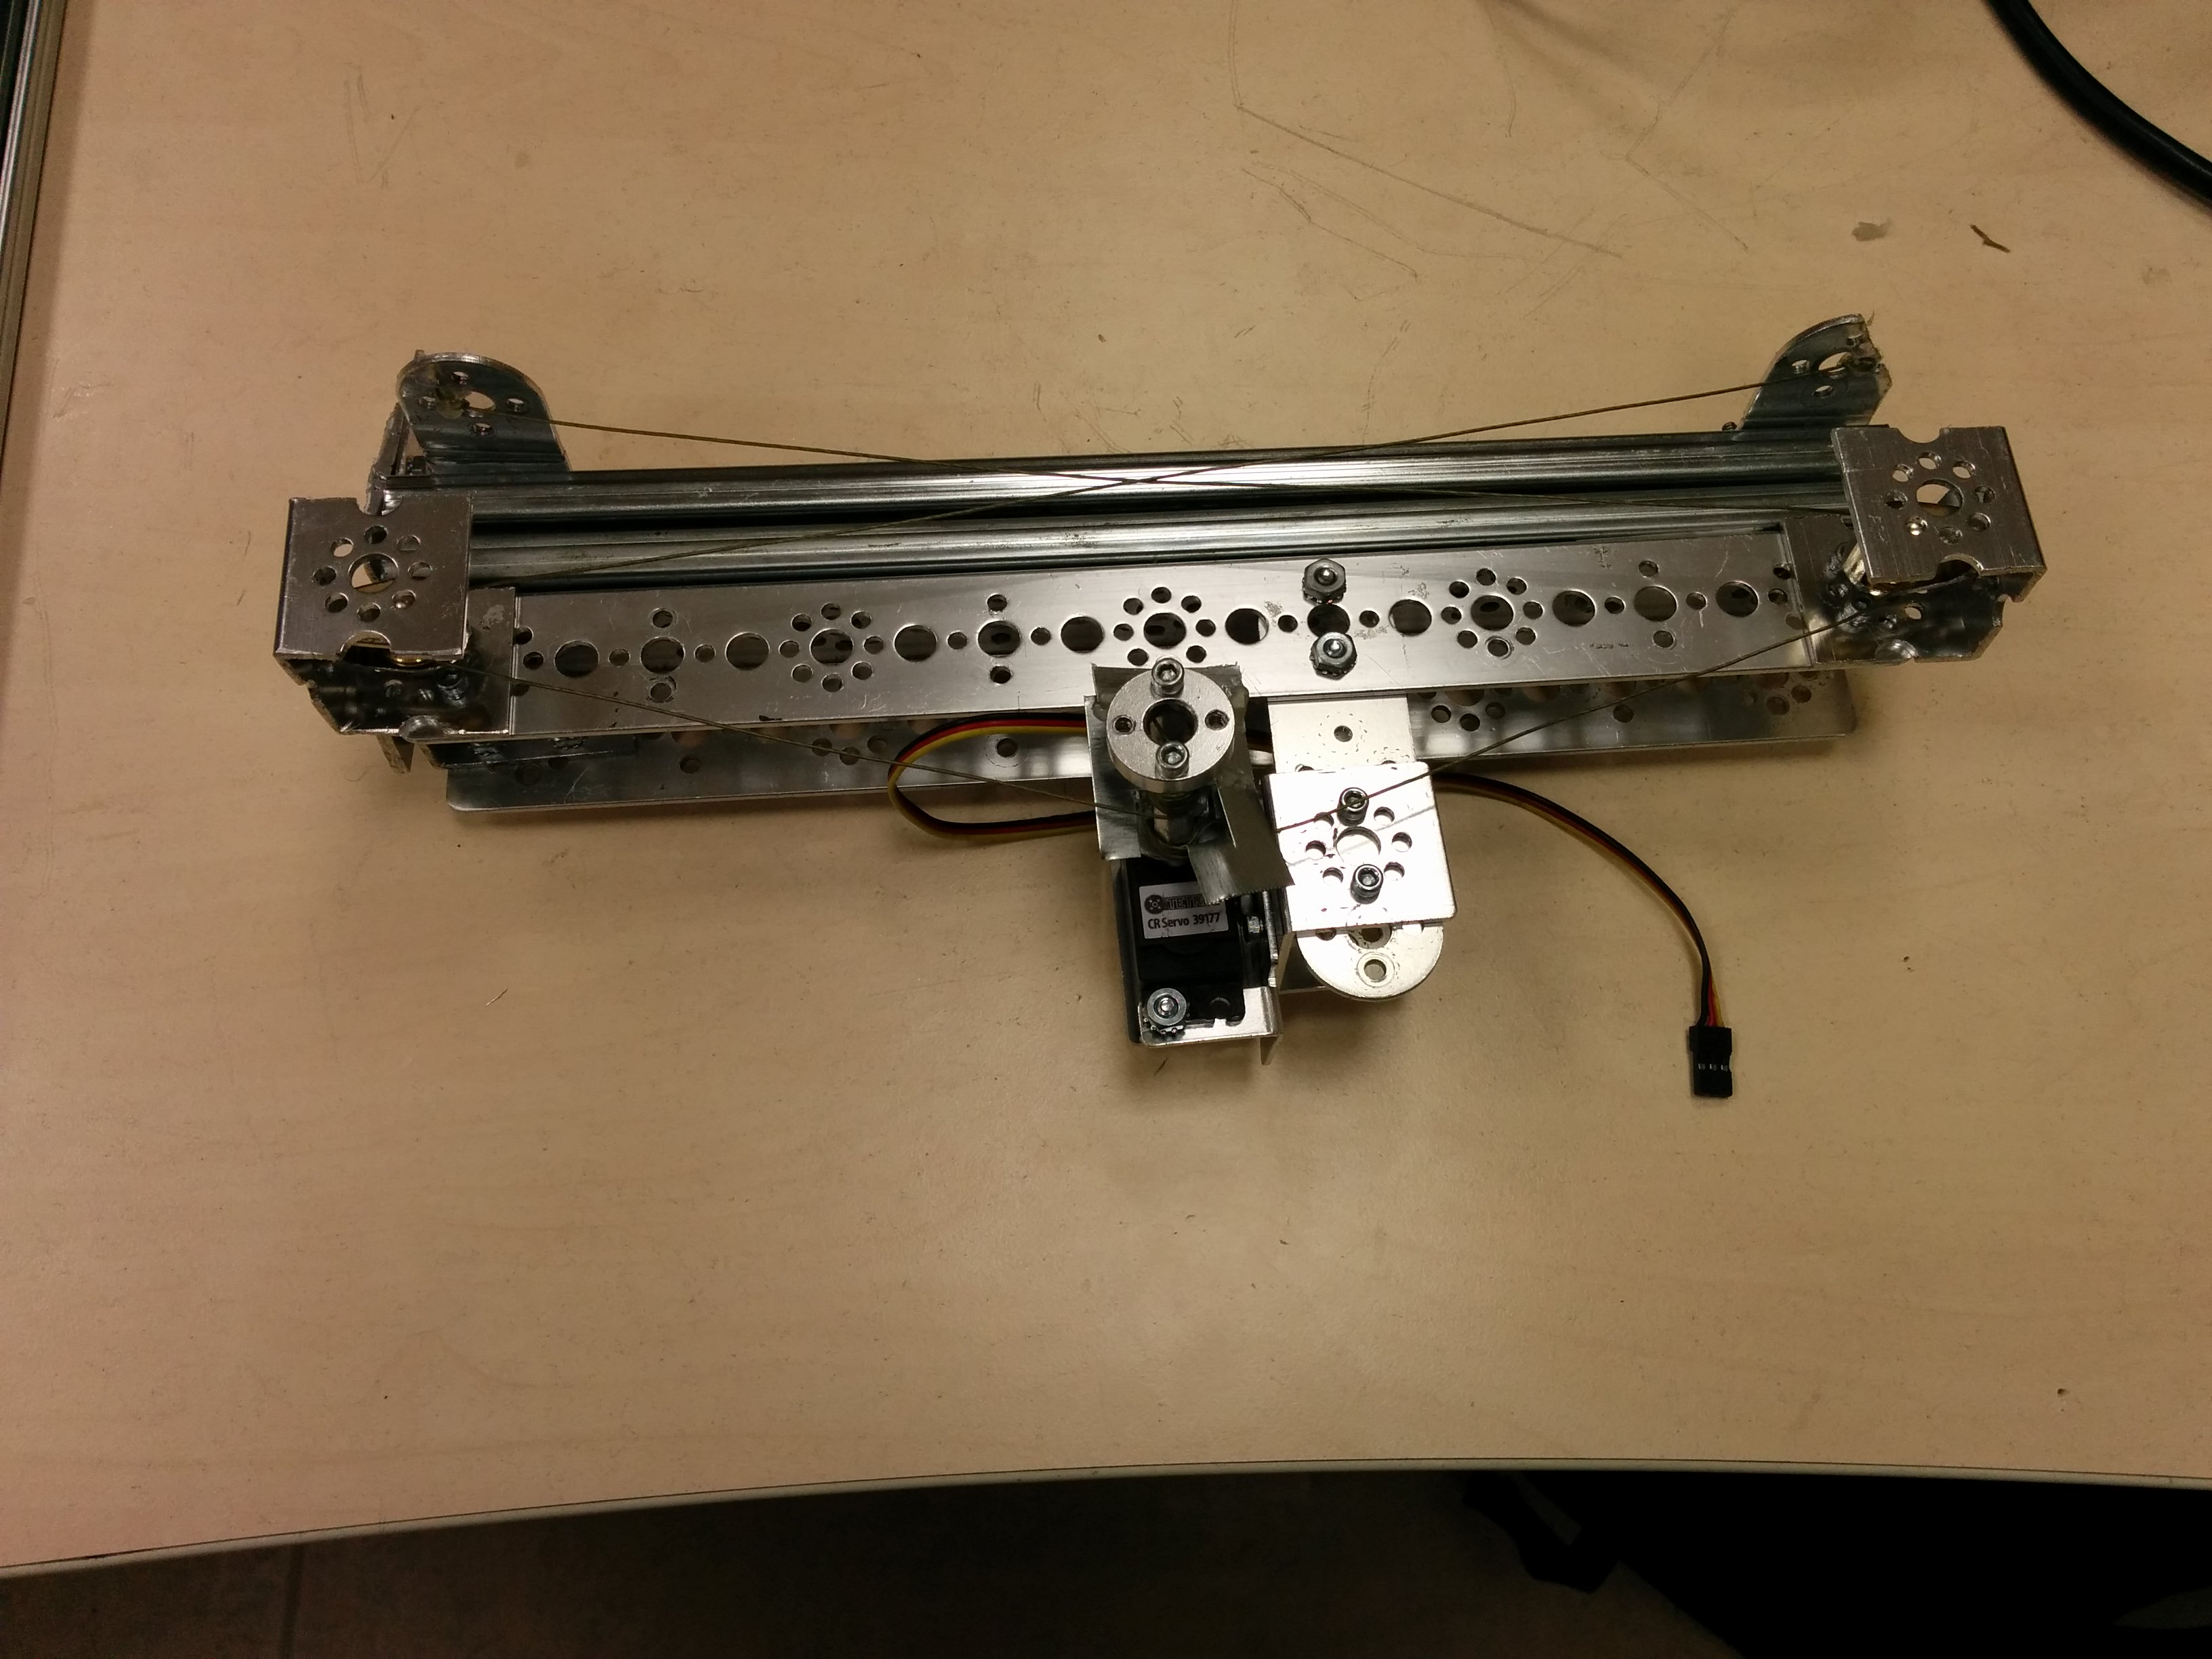
\includegraphics[scale = 0.05]{3Engineering/6Specifications_for_modules/bucket/images/06}}
  		\caption{Construction of line and pulling it servo}
  	\end{minipage}
  	\hfill
  	\begin{minipage}[h]{0.47\linewidth}
  		\center{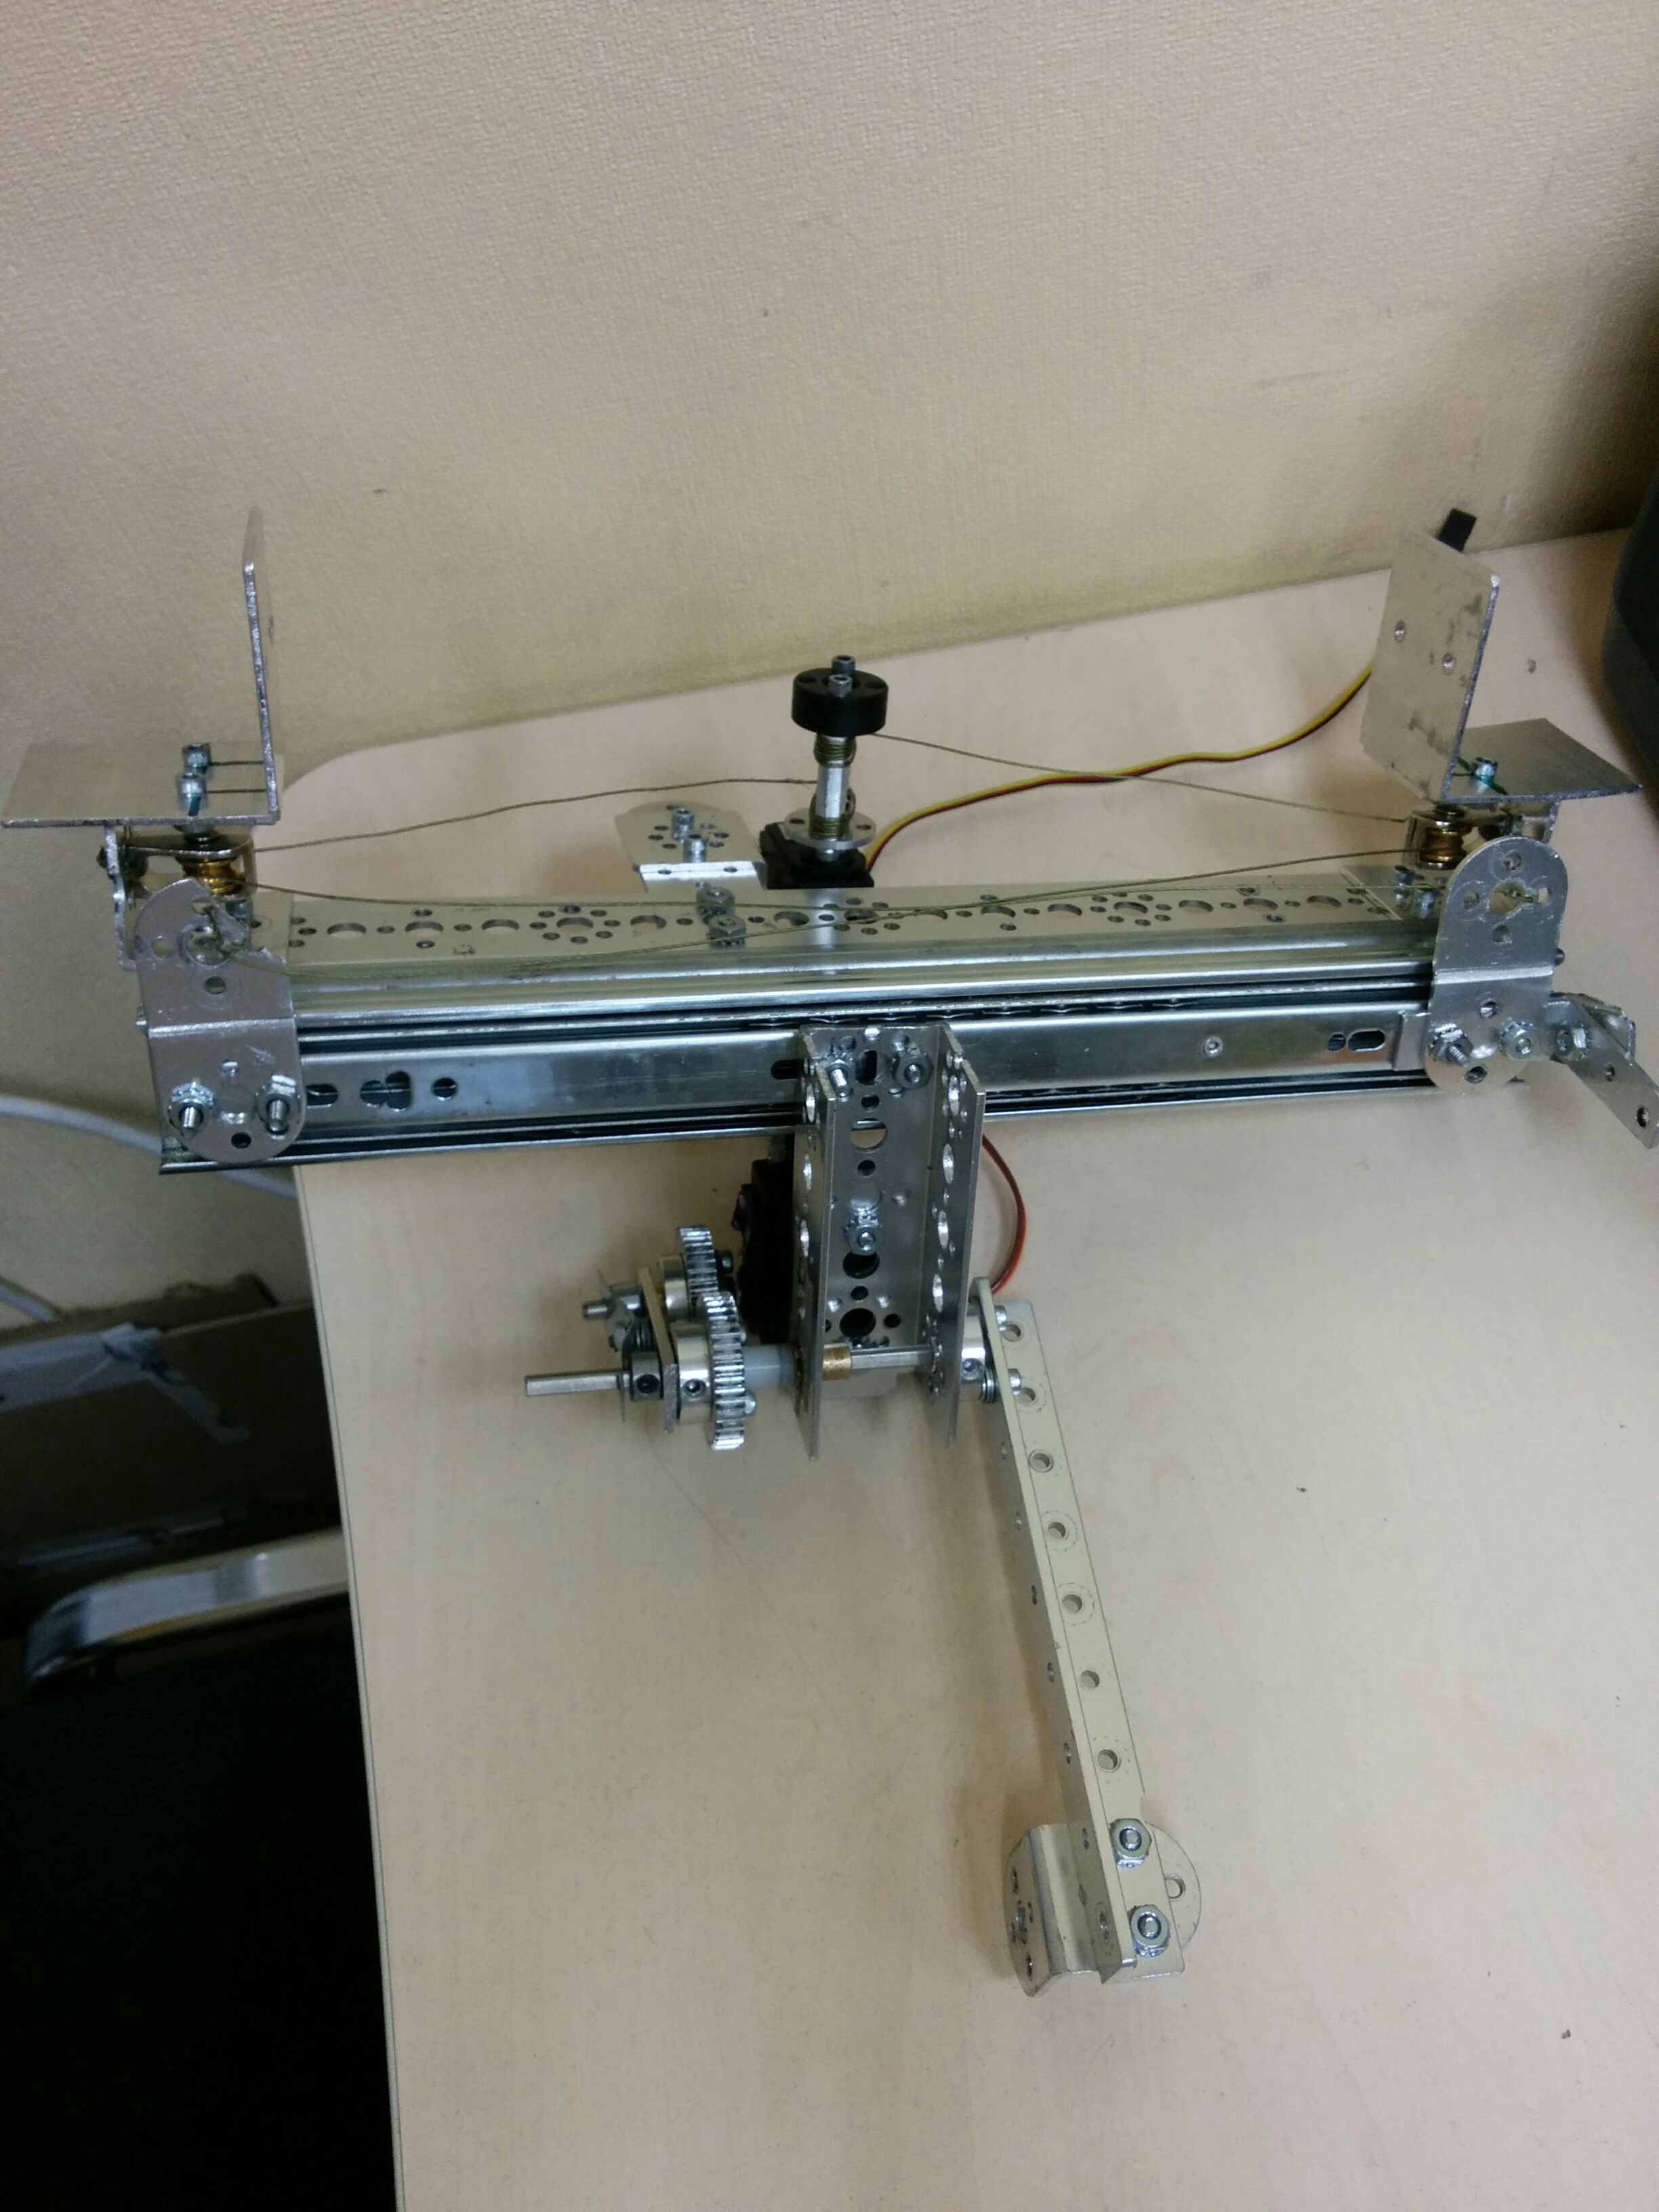
\includegraphics[scale = 0.05]{3Engineering/6Specifications_for_modules/bucket/images/07}}
  		\caption{Final construction of the slats}
  	\end{minipage}
  \end{figure}
  \item The last done part of module is closing mechanism. The difficalty in it is that axis of servo has to be as close as possible to the front-top edge of bucket.
  
  \begin{figure}[h]
  	\begin{minipage}[h]{1\linewidth}
  		\center{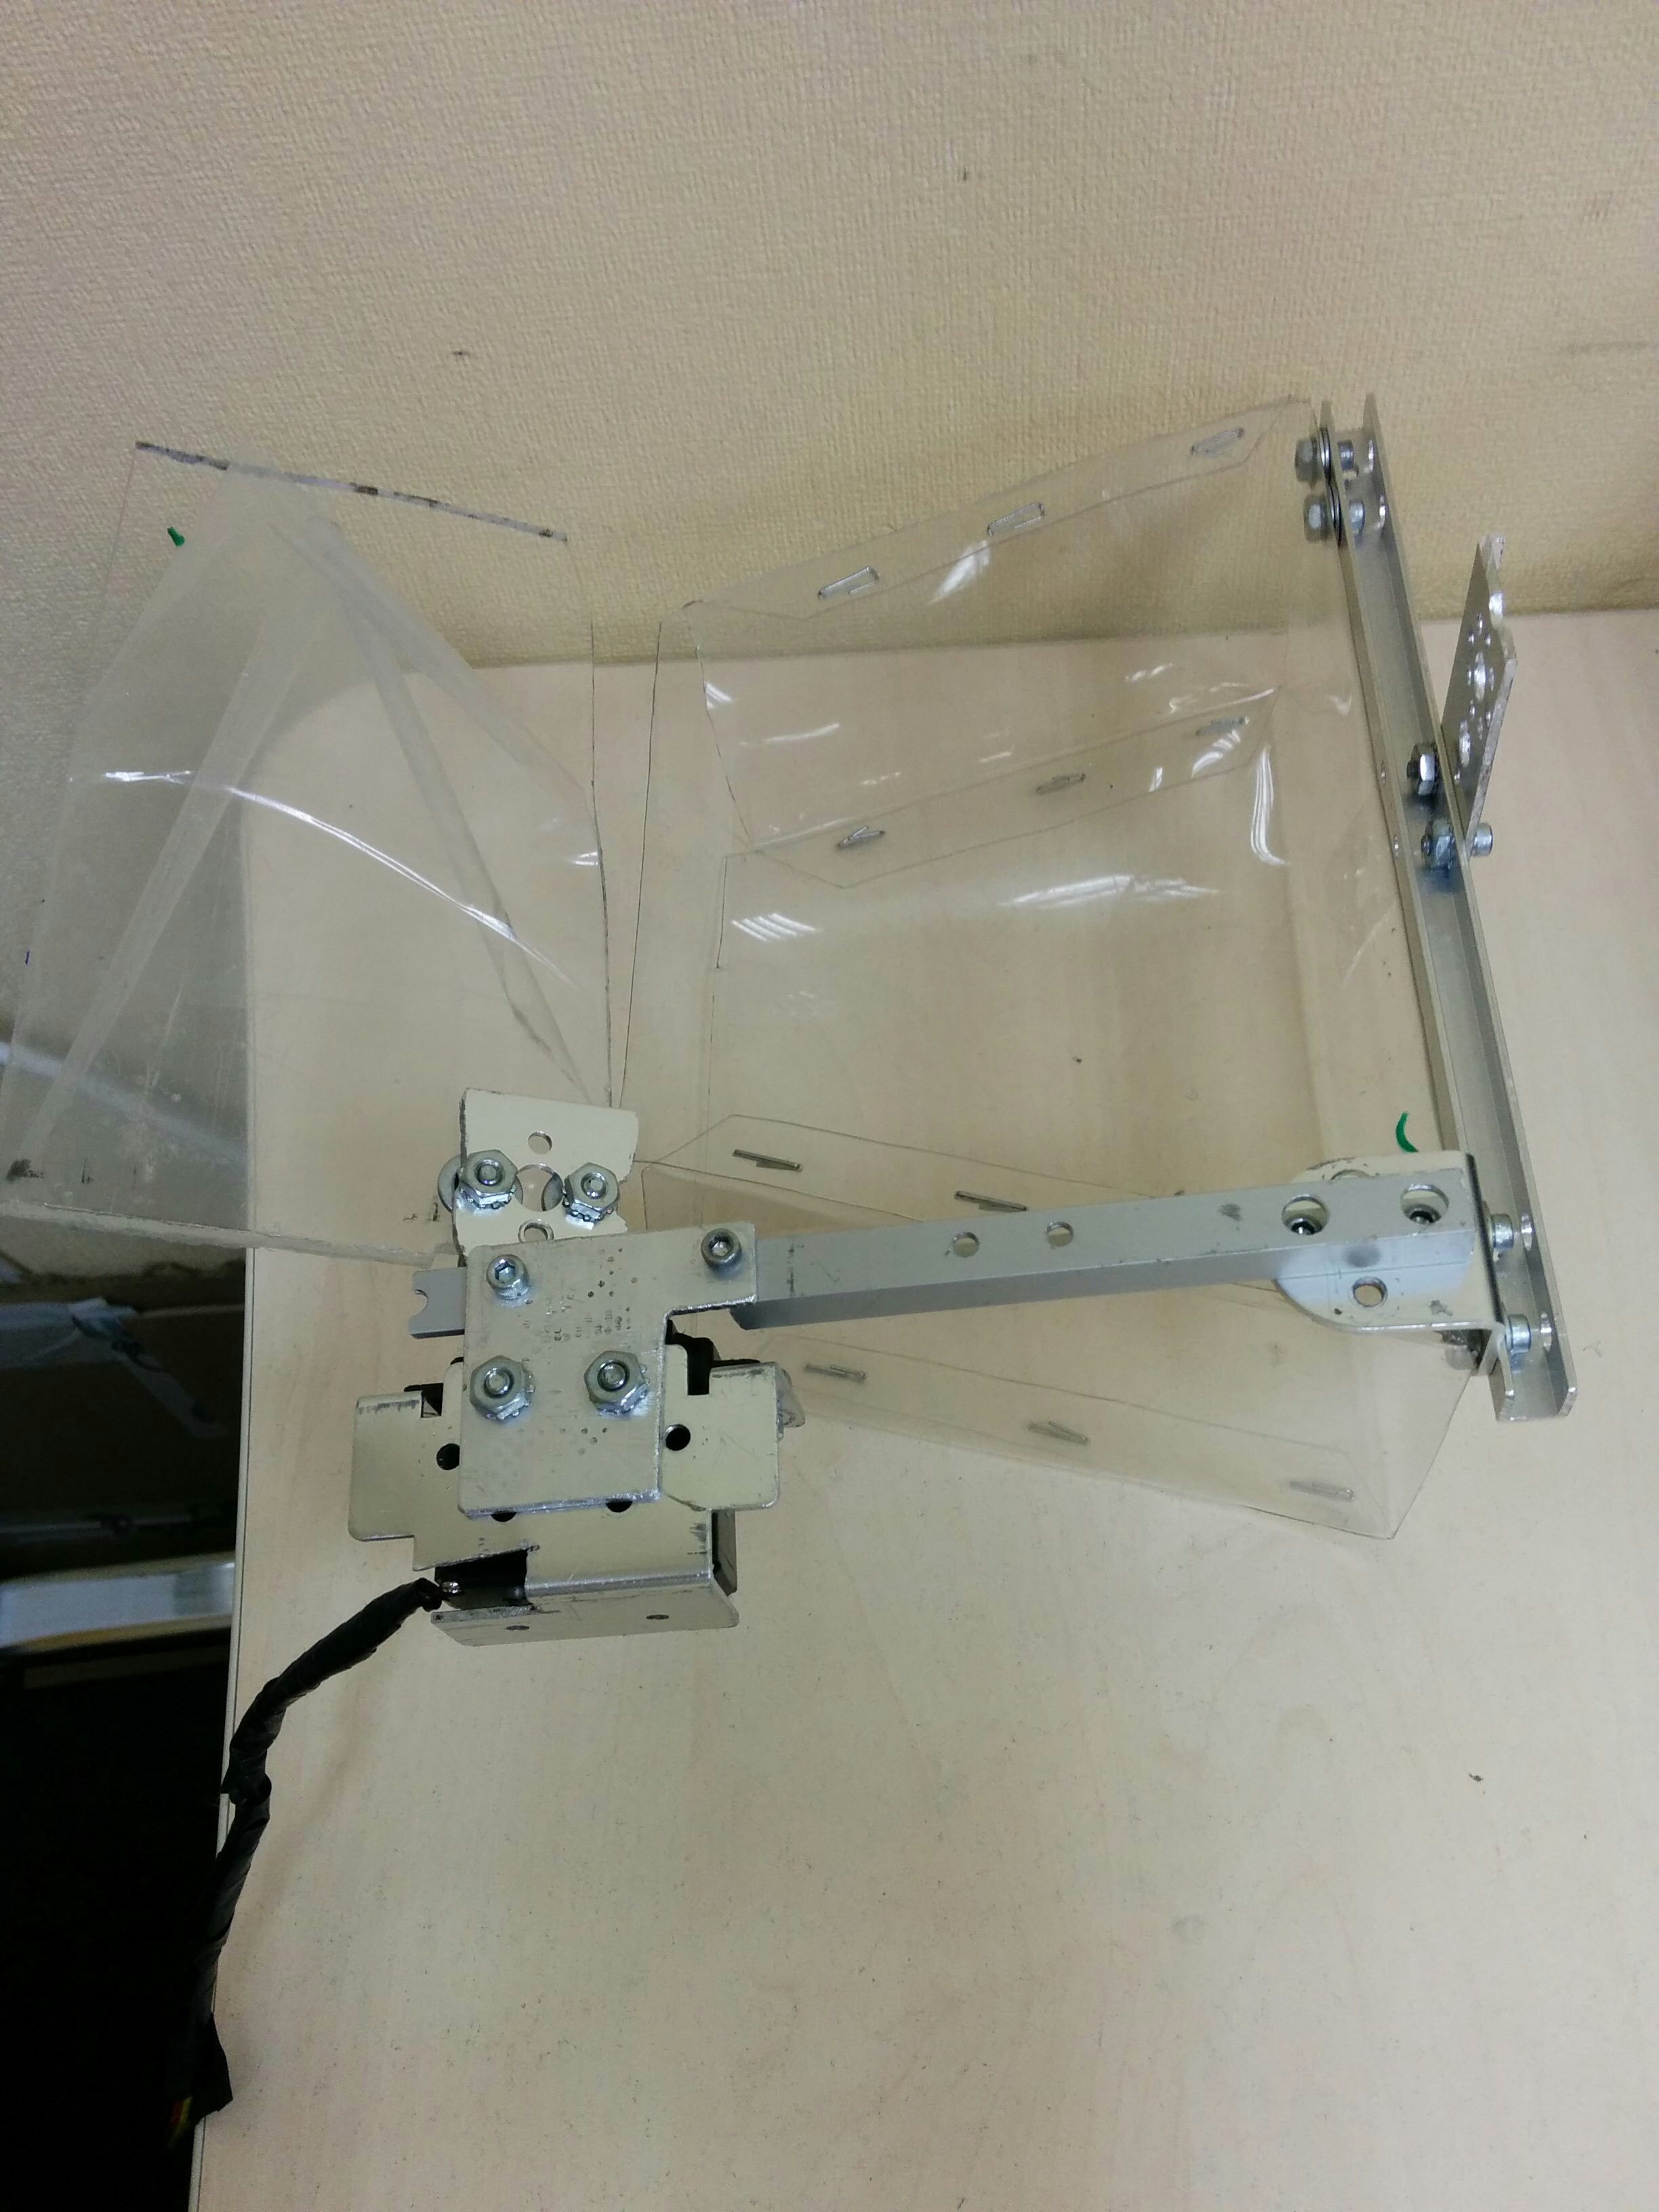
\includegraphics[scale = 0.05]{3Engineering/6Specifications_for_modules/bucket/images/08}}
  		\caption{Final construction of the bucket with closing mechanism}
  	\end{minipage}
  \end{figure}
  
  \end{enumerate}	